\documentclass[main.tex]{subfiles}
\begin{document}



\chapter{Hauptsätze der mehrdimensionalen Integralrechnung}


\section{In 2 Dimensionen}

Wir treffen folgende Aussagen prototypisch für höhere Dimensionen.

\subsection{Divergenz}

\begin{Beispiel}[Luftfluss durch das HG (2D oder 3D)]
  Wir definieren uns den Fluss $f$als Skalarprodukt zwischen dem Normalenvektor auf eine Wand und dem Luftfluss. Dann gilt für den Gesamtfluss:
  $$F = \int_{\partial HG} f = \int_{HG} \text{Quellenstärke}$$
  Allgemein betrachten wir:

  $F$, ein Vektorfeld auf $U \subseteq \R^n$ und $B\subseteq U$ kompakt mit glattem Rand $\partial B$.
\end{Beispiel}

\begin{Definition}[Divergenz]
  Sei $U \subseteq \R^n$ offen und $F: U \to \R^n$ ein stetig differenziebares Vektorfeld. Die \textbf{Divergenz} (Quellenstärke) von $F$ ist die Funktion
  $$\begin{aligned}
    div(F): U & \to \R \\
    (x) & \mapsto tr (DF(x)) = \sum \limits_{i=1}^n \dfrac{\partial}{\partial x_i} F_i
  \end{aligned}$$
\end{Definition}

\begin{Beispiel}
  $$F: \R^2 \to \R^2 \quad F(x) = x$$
  \begin{center}
    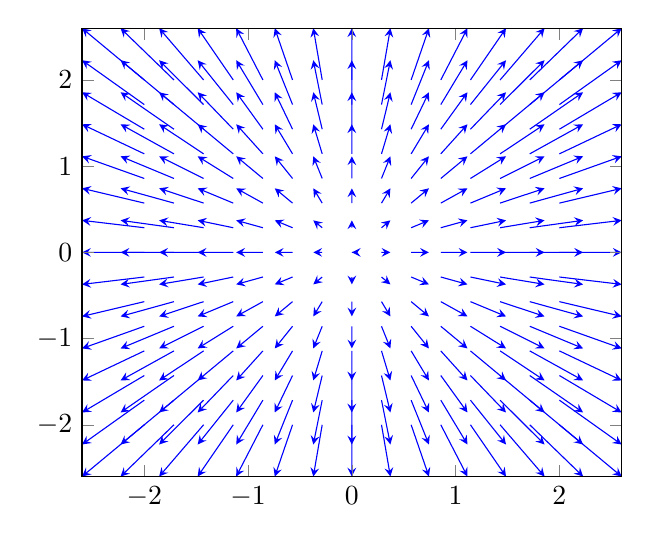
\begin{tikzpicture}
      \begin{axis}[
          domain=-2:2,
          view={0}{90},
          axis background/.style={fill=white},
      ]

          \addplot3[blue,
              quiver={
               u={x},
               v={y},
               scale arrows=0.3,
              },
              -stealth,samples=15]
                  {1};
      \end{axis}
    \end{tikzpicture}
  \end{center}
  Wir haben also
  $$div(F(x)) = tr(id:\R^2 \to \R^2) = tr(E_2) = 2 = \dfrac{\partial}{\partial x_1}F_1(x) + \dfrac{\partial}{\partial x_2}F_2(x) = 1 + 1$$
  Wir können auch haben:
  $$F: \R^2 \to \R^2 \quad F(x) = (1,2)$$
  \begin{center}
    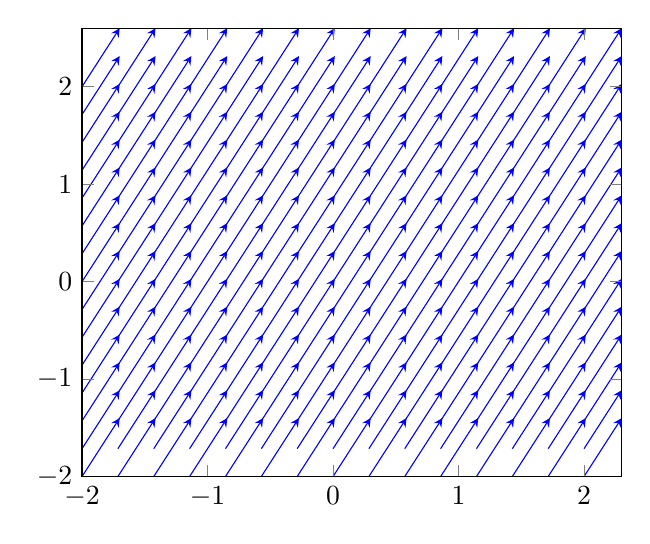
\begin{tikzpicture}
      \begin{axis}[
          domain=-2:2,
          view={0}{90},
          axis background/.style={fill=white},
      ]

          \addplot3[blue,
              quiver={
               u={1},
               v={2},
               scale arrows=0.3,
              },
              -stealth,samples=15]
                  {1};
      \end{axis}
    \end{tikzpicture}
  \end{center}
  Hier gilt
  $$DF(x) = 0 \Rightarrow div(F) = 0$$
\end{Beispiel}

Nun wollen wir also ein Integral über den Rand, einer Jordan-messbaren Menge berechnen. Wir werden uns in den Dimensionen hocharbeiten:

\begin{Definition}[Flussintegral]
  Sei $\gamma: [a,b] \to \R^2$ (stückweise) stetig differenziebar.

  Wir nehmen uns $n_\gamma(t) = (\gamma_2'(t),-\gamma_1'(t))$ und nennen dies den \textbf{Normalenvektor} an den Pfad $\gamma$ an der Stelle $t$. Dieser hat eine eindeutige Richtung.

  Sei nun $F : U \to \R^2$ stetig. Das \textbf{Flussintegral} von $F$ durch $\gamma$ ist
  $$\int_\gamma F dn_\gamma = \int_a^b <F(\gamma(t)),n\gamma(t)> dt = \int F \times \gamma dt$$
\end{Definition}

\begin{Bemerkung}
  Es gilt offensichtlich, dass $<v,n_\gamma(t)> = v \times \gamma(t)$, aber wir werden diese Darstellung nicht weiter verwenden.
\end{Bemerkung}

Skizzenmäßig wollen wir zeigen.

\begin{Theorem}
  Sei $U \subseteq \R^2$ offen, $B \subseteq U$ beschränkt, zusammenhängend und mit glattem Rand und sei weiter $F: U \to \R^2$ von Klasse $\mathcal{C}^1$.
  $$\int_B div(F(x))dx = \underbrace{\int_{\partial B} F dn}_{Flussintegral} = \int_\gamma f dn_\gamma$$
  für eine Kurve $\gamma:[a,b] \to U$, die $\partial B$ parametrisiert.

  (glatt, wassisdas?)
\end{Theorem}

Das ist weiterhin unkonkret, und in Teilen schlecht definiert, aber erlaubt uns zumindest, manche elementaren Fälle darzustellen. (zum Beispiel den Rand eines 2D-Rechtecks). Wir können schon einmal festhalten:

\begin{Theorem}
  Sei $U \subseteq \R^2$ offen und  $F: U \to \R^2$ von Klasse $\mathcal{C}^1$. Sei $B = [a,b] \times [c,d] \subseteq U$ ein Rechteck. Dann gilt
  $$\int_B div(F(x)) dx = \int_{\partial B} F dn$$
\end{Theorem}

\begin{Beweis}
  Der Rand von $B$ ist parametrisiert (?) durch die Kurve $\gamma$, die sich aus den folgenden 4 Kurven zusammensetzt:
  $$\gamma : \left\{ \begin{aligned}
    \gamma_u : [a,b] \to U & \quad & \gamma_u(t) = (t,c) \\
    \gamma_r : [c,d] \to U & \quad & \gamma_r(t) = (b,t) \\
    \gamma_o : [a,b] \to U & \quad & \gamma_o(t) = (a+b -t,d) \\
    \gamma_l : [c,d] \to U & \quad & \gamma_l(t) = (a,c+d -t)
  \end{aligned}\right.
  \Rightarrow n_\gamma : \left\{ \begin{aligned}
    n_{\gamma_u}(t) & = (0,-1) \\
    n_{\gamma_r}(t) & = (1,0) \\
    n_{\gamma_o}(t) & = (0,1) \\
    n_{\gamma_l}(t) & = (-1,0)
  \end{aligned}\right.$$
  Also ist das Flussintegral:
  $$\begin{aligned}
    \underbrace{\int_a^b <F(t,c),(0,-1)> dt}_{\gamma_u, n_{\gamma_u}} & +
    \underbrace{\int_c^d <F(b,t),(1,0)> dt}_{\gamma_r, n_{\gamma_r}} \\
    + \underbrace{\int_a^b <F(a+b - t,d),(0,1)> dt}_{\gamma_o, n_{\gamma_o}} & +
    \underbrace{\int_a^b <F(a ,c + d - t),(-1,0)> dt}_{\gamma_l, n_{\gamma_l}}
  \end{aligned}$$
  Nun formen wir um mit der Substitution: $a+ b - t \rightsquigarrow t$ und $c + d - t \rightsquigarrow t$:
  $$\begin{aligned}
    = & \int_a^b F_2 (t,d) - F_2 (t,c) dt + \int_c^d F_1(b,t) - F_1(a,t)dt \\
    \stackrel{\scriptscriptstyle Hauptsatz}{=} & \int_a^b \int_c^d \dfrac{\partial}{\partial x_2} F_2(t,y) dy dt + \int_a^b \int_c^d \dfrac{\partial}{\partial x_1} F_1(x,t)dx dt \\
    \stackrel{\scriptscriptstyle Fubini}{=} & \int_B \dfrac{\partial}{\partial x_1} F_1(x,y) + \dfrac{\partial}{\partial x_2} F_2(x,y) d(x,y) \\
    = & \int_B div(F) dx
  \end{aligned}$$
\end{Beweis}

\begin{Bemerkung}
  Damit sind die meisten Mengen weiterhin außer Reichweite, aber wir können immerhin auch zusammengesetzte Rechtecke betrachten:
  \incfig{zusammengesetzte-rechtecke}
  Für $B := B_1 \cup B_2 \cup B_3$ gilt
  $$\int_B div(F) = \int_{B_1} div(F) + \int_{B_2} div(F) + \int_{B_3} div(F)$$
  Außerdem müssen wir betrachten, dass die Raänder sich gegenseitig auscanceln (sie zeigen jeweils im Mathematisch positiven Sinne um das Rechteck herum):
  $$\int_{\partial B} = \int_{\partial B_1} + \int_{\partial B_2} +\int_{\partial B_3}$$
\end{Bemerkung}

\begin{Theorem}
  Sei $U \subseteq \R^2$ offen, $F: U \to \R^2$ von Klasse $\mathcal{C}^1$ und $Q = [a,b] \times [c,d] \subseteq U$. Sei $\varphi: [a,b] \to [c,d]$ stetig differenziebar mit beschränkter Ableitung.

  Für $B := \{(x,y) \in \Q \mid y \leq \varphi(x)\}$ gilt
  $$\int_B div(F(x)) = \int_{\partial B} F dn$$
  \incfig{theorem-divergenz-1}
\end{Theorem}

\begin{Beweis}
  $\partial B$ ist parametrisiert durch 4 Pfade: $\gamma_u,\gamma_l,\gamma_r$ wie für Rechtecke und
  $$\gamma_o(t) = (a+b-t,\varphi(a+b-t)) \quad \text{für $t \in [a,b]$}$$
  also haben wir $n_{\gamma_o}(t) = (-\varphi'(a+b-t),1)$
  $$\begin{aligned}
    \int_{\partial B} F dn & = \underbrace{-\int_a^b F_2(t,c)dt}_{unten} + \underbrace{\int_c^{\varphi(b)} F_1(b,t)dt}_{rechts} - \underbrace{\int_a^b F_1(t,\varphi(t)) \cdot \varphi'(t)dt + \int_a^b F_2 (t,\varphi(t))dt}_{oben} \\
    & - \underbrace{\int_c^{\varphi(a)} F_1(a,t)dt}_{links}
  \end{aligned}$$
  \incfig{theorem-divergenz-2}
  Wir nehmen die Maschenweite $\delta > 0$ klein. Wir unterteilen $A = \bigcup \limits_{i=1}^N A_i$ und wenden eine ganze Menge Abschätzungen an:
  $$\int_B div(F(x)) = \int_{\partial B} F dn \Leftrightarrow \left|\int_B div(F(x)) - \int_{\partial B} F dn \right| \leq \varepsilon = 0$$
  $$\begin{aligned}
    \left|\int_B div(F(x)) - \int_{\partial B} F dn \right| & = \left|\int_B div(F(x)) - \int_A div(F(x)) - \int_{\partial B} F dn + \int_A div(F(x)) \right| \\
    & \text{weil } \int_A div(F(x)) = \int_{\partial A} F dn \\
    & \stackrel{\scriptscriptstyle DUG}{\leq} \underbrace{\left|\int_B div(F(x)) - \int_A div(F(x))\right|}_{\leq vol(A \Delta B) \cdot ||div(F)||_\infty} + \underbrace{\left| \int_{\partial B} F dn + \int_A div(F(x)) \right|}_{} \\
    & \leq vol(A \Delta B) \cdot ||div(F)||_\infty + \\
    & \leq \varepsilon \cdot M +
  \end{aligned}$$
  Ok ich gebe auf... etc. etc. etc...
\end{Beweis}

\begin{Bemerkung}
  Die Aussage des Satzes gilt auch für Bereiche $B$: Im Allgemeinen können wir nämlich die meisten Mengen als Graphen darstellen. Diese müssen wir nur noch adäquat definieren.
\end{Bemerkung}

\begin{Definition}[Glatt berandeter Bereich]
  Eine abgeschlossene Teilmenge $B \subseteq \R^n$ heißt \textbf{glatt berandeter Bereich}, falls es zu jedem Punkt $p \in B$ eine Umgebung $U$ von $p \in \R^n$ und einen Diffeomorphismus $\varphi: U \to V \subseteq \R^n$ mit
  $$\varphi(U \cap B) = \{y \in V \mid y_n \leq 0\}$$
  existiert.

  Der Rand von $B$ ist somit eine Teilmannigfaltigkeit von Dimension $n - 1$
\end{Definition}

\begin{Beispiel}[Motivierung]
  Sei folgende Menge $B$ und ein Punkt $P \in \partial B$. Wir wollen $F$ bei $\partial B$ berechnen. Für
  $$F = \left\{\begin{array}{c c c}
    F(x) & \text{falls} & x \in Q \\
    0 & \text{sonst}
  \end{array}\right.$$
  \incfig{theorem-divergenz-bsp}
  Nun haben wir
  $$\begin{aligned}
    \int_B div(F) dx & = \int_{\partial B} F dn \\
    & \text{aber auch:} \\
    & = \int_{B \cap Q} div(F) dx = \int_{\partial B \cap Q} F dn = \int_{\partial (B \cap Q)} F dn
  \end{aligned}$$
  Schreibe nun $F$ als $F_1 + F_2 + ... + F_N$ mit $supp(F_i) \subsetneq Q_i$. Dann gilt
  $$\int_B div(F) dx = \sum \limits_{i=1}^N \int_B div(F_i) dx = \int_{B \cap Q_i} F_i dx = \sum \limits_{i=1}^N \int_{\partial B \cap Q_i} F_i dn = \int_{\partial B} F dn$$
  Angenommen wir finden $\eta_1 , ..., \eta_N : \R^2 \to \R$ glatt, mit $supp(\eta_i) \subseteq Q_i$ und $\eta_1 + ...+ \eta_N = 1$ in einer Umgebung von $B$, dann kann man schreiben: $F_i = \eta_i \cdot F$.
\end{Beispiel}

\begin{Theorem}
  Sei $K \subseteq \R^n$ kompakt, sei $U_1, ..., U_N$ eine offene Überdeckung von $K$. Dann existieren glatte Funktionen $\eta_0,\eta_1 , ..., \eta_N: \R^n \to [0,1]$ mit
  \begin{enumerate}
    \item $supp(\eta_0) \subseteq \R^n \backslash K$
    \item $supp(\eta_i) \subseteq U_i$ für $1 \leq i \leq N$
    \item $\eta_0 + \eta_1 + ... \eta_N = 1$
  \end{enumerate}
\end{Theorem}
\begin{Beweis}
  Setze $U_0 = \R^n \backslash K$. Definiere Abstandsfunktionen
  $$\begin{aligned}
    d_i : \R^n & \to \R_{\geq 0} \\
    d_i(x) & = \inf\{||x-y||\mid y \in \R^n \backslash U_i\}
  \end{aligned}$$
  Konkret bedeutet das: $d_i (x) \geq 0$ für $x \in U_i$ und $d_i(x) = 0$ sonst.

  Sei $\lambda > 0$ eine Lebesgue-Zahl zur Überdeckung $U_0,...,U_N$ von $\R^n$. Setze
  $$\tilde{h_i}(x) = \min\left\{0,d_i(x) - \frac{\lambda}{2}\right\} \quad i \leq N$$
  Für jedes $x \in \R^n$ existiert $i \leq N$ mit $h_i(x) > 0$. Also ist
  $$H(x) := \tilde{h_0}(x) + ... + \tilde{h_N}(x)> 0$$
  Setze
  $$\begin{aligned}
    h_i : \R^n & \to [0,1] \\
    h_i(x) & = \dfrac{\tilde{h_i}(x)}{H(x)}
  \end{aligned}$$

  und dann gilt
  $$supp(h_i) {\color{olive}  + B\left(0,\frac{\lambda}{4}\right)}\subseteq U_i \quad \text{und} \quad  h_0 + ... + h_N = 1$$
  \textbf{ABER:} diese $h_i$ sind nicht glatt, und können deshalb nicht als $\eta$ aus dem Satz fungieren. Dies benötigt noch etwas Vorarbeit:

  Glücklicherweise ist $h_i$ so definiert, so dass der Träger in $U_i$ einen 'Puffer' hat (in grün nachgetragen). Also können wir $h_i$ glätten:

  Sei $\psi : \R^n \to \R_{\geq 0}$ glatt, mit
  $$supp(\psi) \subseteq B\left(0,\frac{\lambda}{4}\right) \quad \text{und} \quad \int_{\R^n} \psi(x) dx = 1$$
  und setze $\eta_i(x) = \int_{\R^n} \psi(y) \cdot h_i(x-y) dy$, die Glättung in jeder Variablen.

  Also ist
  \begin{enumerate}
    \item $\eta_i$ glatt
    \item $supp(\eta_i) \subseteq U_i$
    \item $$\begin{aligned}
      \sum \limits_{i=0}^N \eta_i & = \sum \limits_{i=0}^N \psi \cdot h_i \\
      & = \psi \cdot \sum \limits_{i=0}^N h_i \\
      & = \psi \cdot 1 \\
      & = \int_{\R^n} \psi(y) \cdot 1 dy \\
      & = 1
    \end{aligned}$$
  \end{enumerate}
\end{Beweis}

\begin{Bemerkung}[Zusammenhang zwischen $tr$ und $div$]
  Sei $F: U \subseteq \R^n \to \R^n$ ein Vektorfeld der Klasse $\mathcal{C}^1$. Wir hatten definiert
  $$div F(x) = tr \, DF(x) = \sum \limits_{i=1}^n \partial_i F_i(x)$$
  Wenn wir den 2D Fall betrachten, haben wir $F(x) = (F_1(x),F_2(x))$ (horizontal und vertikal).

  Bilden wir nun die Ableitung unseres reorientierten Vektorfeldes haben wir:
  $$DF(x) = \begin{pmatrix}
    \partial_1 F_1(x) & \partial_2 F_1(x) \\ \partial_2 F_1(x) & \partial_2 F_2(x)
  \end{pmatrix} = \begin{pmatrix}
    \partial_1 F_1(x) & 0 \\ 0 & \partial_2 F_2(x)
  \end{pmatrix}$$
  Wenn wir nun die Quellenstärke des Eingeschlossenen Quadrats finden wollen, müssen wir die Differenz ziwschen dem eingehenden und dem ausgehenden Fluss berechnen. Das können wir nun komponentenweise. Und wir erhalten: $\partial_1 F_1(x) + \partial_2 F_2(x) = tr \, DF(x)$.
\end{Bemerkung}

\begin{Definition}[Parametrisierung des Randes]
  Sei $B \subseteq \R^2$ (ohne Voraussetzung) mit Rand $\partial B = \overline{B} \backslash \mathring{B}$.

  Eine \textbf{(reguläre, positiv orientierte) Parametrisierung des Randes von $B$} ist eine \textbf{endliche} Kollektion von Kurven
  $$\gamma_k : [a_k,b_k] \to \R^2 \quad k \leq N$$
  mit folgenden Eigenschaften:
  \begin{enumerate}
    \item Überdeckend:
      $$\bigcup \limits_{k=1}^N \gamma_k([a_k,b_k]) = \partial B$$
    \item Nicht überschneidend:

      Für $t \in [a_k,b_k]$ und $s \in [a_l,b_l]$ soll gelten
      $$\gamma_k(t) = \gamma_l(s)\Rightarrow \left\{\begin{array}{c c}
        k = l & \\
        \text{oder} & \\
        l \neq k & \text{ und } t \in \{a_k,b_k\} \text{ und } s \in \{a_l,b_l\}
      \end{array}\right.$$
    \item Aufeinanderfolgend:
      $$\A k \leq N \E! l \leq N : \gamma_k(b_k) = \gamma_l(a_l)$$
    \item Regularität:
      $$\gamma_k'(t) \neq 0 \A t \in (a_k,b_k)$$
    \item Orientierung:
      $$\A t \in [a_k,b_k] : \gamma_k(t) - \varepsilon \cdot n_\gamma(t) \in \mathring{B} \A \varepsilon > 0 \text{ klein genug}$$
  \end{enumerate}
  Dies existiert für glatt berandete Bereiche immer.

  \textbf{Notation:}

  Ist $B \subseteq U$ kompakt und $U \subseteq \R^2$ offen. Dann schreibe für $F: U \to \R^2$ von Klasse $\mathcal{C}^1$:
  $$\int_{\partial B} F dt = \sum \limits_{k=1}^N \int_{\gamma_k}F dt = \sum \limits_{k=1}^N \int_{a_k}^{b_k} <F(\gamma_k(t)),\gamma_k'(t)> dt \quad \text{(Arbeitsintegral)}$$
  $$\int_{\partial B} F dn = \sum \limits_{k=1}^N \int_{\gamma_k}F dn = \sum \limits_{k=1}^N \int_{a_k}^{b_k} <F(\gamma_k(t)),n_{\gamma_k}(t)> dt \quad \text{(Flussintegral)}$$
  für eine positiv orientierte, reguläre Parametrisierung des Randes.
  \begin{Theorem}
    Diese Integrale sind unabhängig von der Parametrisierung.
  \end{Theorem}
\end{Definition}

\begin{Beweis}
  Für Arbeitsintegrale haben wir diese Aussage bereits gezeigt.

  Für das Flussintegral betrachten wir
  $$I = \begin{pmatrix}
    0 & -1 \\ -1 & 0
  \end{pmatrix} \qquad I^2 = - id \qquad I^T = -I$$
  Es gilt also:
  $$I \cdot \begin{pmatrix}
    x \\ y
  \end{pmatrix} = \begin{pmatrix}
    y \\ -x
  \end{pmatrix} \qquad I \cdot \gamma'(t) = n_\gamma(t) \qquad <v,Iw> = -<Iv,w>$$
  Also hat man
  $$\begin{aligned}
    \int_\gamma F dn & = \int_a^b <F(\gamma(t)),n_\gamma(t)> dt \\
    & = \int_a^b <F(\gamma(t)),I \cdot \gamma'(t)> dt \\
    & = -\int_a^b <I \cdot F(\gamma(t)),\gamma'(t)> dt \\
    & = \int_\gamma(I\cdot F) dt
  \end{aligned}$$
\end{Beweis}

\begin{Theorem}
  Sei $U \subseteq \R^2$ offen, $B \subseteq U$ glatt berandet und kompakt und $F: U \to \R^2$ ein Vektorfeld der Klasse $\mathcal{C}^1$. Dann gilt
  $$\int_{\partial B} Fdn = \int_B div(F) dx$$
\end{Theorem}

\begin{Beweis}
  Wähle zu jedem $x \in B$ eine Karte $U_x \stackrel{\scriptscriptstyle \varphi_x}{\longrightarrow} V_x$ mit $\varphi_x(U_x \cap B) = V_X \cap \{x \in \R^2 \mid x \leq 0 \}$
  \incfig{theorem-divergenz-beweis}
  OBdA ist $U_x$ ein Rechteck und $B \cap U_x$ der Bereich unter dem Graphen einer Funktion. $B$ kompakt bedeutet, dass wir nur endlich viele Karten betrachten müssen, weil $U_1,...,U_N$ $B$ bereits überecken. Sei $\eta_0,...,\eta_N$ eine glatte Zerlegung der eins, bezüglich dieser Überdeckung. Setze $F_i = \eta_i \cdot F$
  $$\begin{aligned}
    \int_B div(F) dx & = \sum \limits_{i = 0}^N \int_B div(F_i) dx \\
    & \text{weil } supp(F_0) \cap B = \emptyset :\\
    & = \sum \limits_{i = 1}^N \int_B div(F_i) dx \\
    & \text{weil } supp(F_i) \subseteq U_i :\\
    & = \sum \limits_{i = 1}^N \int_{U_i \cap B} div(F_i) dx \\
    & = \sum \limits_{i = 1}^N \int_{\partial B \cap U_i} F_i dx \\
    & = \sum \limits_{i = 1}^N \int_{\partial B} F_i dx \\
    & = \sum \limits_{i = 0}^N \int_{\partial B} F_i dx \\
    & = \int_{\partial B}F dn
  \end{aligned}$$
\end{Beweis}

\begin{Bemerkung}
  Der Satz gilt auch für Bereiche $B \subseteq \R^2$, die 'endlich viele Ecken' haben. Also, die fast überall glatt sind.
\end{Bemerkung}

\begin{Beispiel}[Epizykloide]
  $$B \subseteq \R^2 \text{ kompakt} \qquad \partial B \text{ parametrisierbar}$$
  $$F: \R^2 \to \R \quad F(x)=x \quad DF(x) = id \quad div(F(x)) = 2$$
  Also hat man:
  $$\begin{aligned}
    2 \cdot vol(B) = \int_B div(F) dx & = \int_a^b <\gamma(t),n_\gamma(t)> dt \\
    & = \int_a^b \gamma_1(t)\gamma_2'(t) - \gamma_2(t)\gamma-1'(t) dt
  \end{aligned}$$
  Wir betrachten konkret: (für $m \in \N$)
  $$\gamma(t) = \left(1 + \dfrac{1}{m}\right) \cdot \begin{pmatrix}
    \cos(t) \\ \sin(t)
  \end{pmatrix} + \dfrac{1}{m} \cdot \begin{pmatrix}
    \cos((m+1)t) \\ \sin((m+1)t)
  \end{pmatrix}$$

  \begin{center}
    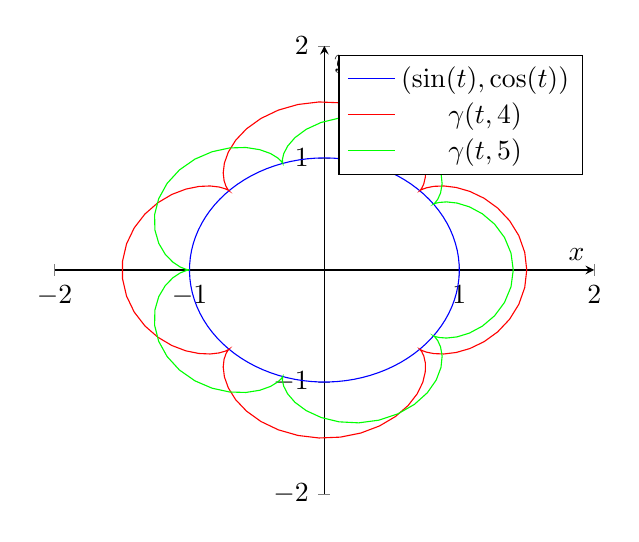
\begin{tikzpicture}
      \begin{axis}[
        axis lines=middle,
        xlabel = {$x$},
        ylabel = {$y$},
        xmin=-2, xmax=2, ymin=-2, ymax=2,
        % legend pos=north west,
        ]
        \newcommand\epix[2]{(1 + 1/#2) * cos(deg(#1)) + 1/#2 * cos(deg((#2 + 1) * #1))}
        \newcommand\epiy[2]{(1 + 1/#2) * sin(deg(#1)) + 1/#2 * sin(deg((#2 + 1) * #1))}

        \addplot[blue,samples=100,domain=0:2*pi]
        ({sin(deg(x))}, {cos(deg(x))});
        \addlegendentry{$(\sin(t),\cos(t))$}
        \addplot[red,samples=100,domain=0:2*pi]
        ({\epix{x}{4}}, {\epiy{x}{4}});
        \addlegendentry{$\gamma(t,4)$}
        \addplot[green,samples=100,domain=0:2*pi]
        ({\epix{x}{5}}, {\epiy{x}{5}});
        \addlegendentry{$\gamma(t,5)$}
      \end{axis}
    \end{tikzpicture}
  \end{center}

  Und man erhält
  $$\begin{aligned}
    vol(B) & = \dfrac{1}{2}v\int_0^{2\pi} \dfrac{(m+1)^2}{m^2} + \dfrac{m + 1}{m^2} + \underbrace{\alpha \cdot \cos(t)\cos((m+1)t) + \beta \cdot \sin(t)\sin((m+1)t)}_{\Rightarrow 0} dt \\
    & = \pi \cdot \dfrac{(m+1)(m+2)}{m^2}
  \end{aligned}$$
\end{Beispiel}

\subsection{Rotation}

\begin{Theorem}[Satz von Green]
  Sei $B \subseteq U \subseteq \R^2$ glatt berandet und sei $F : U \to \R^2$ von Klasse $\mathcal{C}^1$. Dann gilt
  $$\int_{\partial B} F dt = \int_B div(-I\cdot F)dx := \int_B rot(F) dx$$
  (Also ist $rot(F)(x) = \partial_2 F_1(x) - \partial_1 F_2(x)$)
\end{Theorem}

\begin{Beweis}
  $$-I \cdot F = (-F_2 \quad F_1) \qquad div(-I \cdot F) = -\partial_1 F_2 + \partial_2 F_1 = rot(F)$$
\end{Beweis}

\begin{Definition}[Rotationsfreies Vektorfeld]
  Ein Vektorfeld $F: U \to \R$ heißt \textbf{rotationsfrei}, falls
  $$rot(F) = 0 \quad \Leftrightarrow \quad \partial_2 F_1 = \partial_1 F_2 \quad \Leftrightarrow \quad F \text{ erfüllt die Integrabilitätsbedingung}$$
\end{Definition}


\section{Oberflächenintegrale}

\subsection{Flächen (im $\R^3$)}

Wir betrachten im Folgenden spezielle Fälle:
\begin{enumerate}
  \item $B \subseteq \R^3$ glatt berandet und kompakt. Dann hat $B$ eine Oberfläche $\partial B$. Wir betrachten dann Felder oder Flüsse auf $U \supset B$.
  \item Eine Fläche mit Rand in $\R^3$ und dann Felder und Flüsse auf ebendieser Fläche.
\end{enumerate}

Zur Erinnerung
\begin{Definition}[Teilmannigfaltigkeit]
  Teilmannigfaltigkeiten von $\R^3$ der Dimension 2 sind: $X \subseteq \R^3$ mit
  $$\A p \in X \E \text{ eine Karte } \varphi: U \to V \mid \varphi(U \cap X) = V \cap \R^2$$
  Sei $(U_i \stackrel{\varphi_i}{\longrightarrow} V_i \subseteq \R^3)_{i \in I}$ ein Atlas von $X$.

  Nenne
  $$\begin{array}{c c c c}
    \alpha_{ij}: & \varphi(U_i \cap U_j) & \stackrel{\varphi_j \circ \varphi_i^{-1}}{\longrightarrow} & \varphi_j(U_i \cap U_j) \\
    & \subseteq & & \subseteq \\
    & V_i & & V_j
  \end{array}$$
  \textbf{Transitionsabbildung}.
\end{Definition}

\begin{Definition}
  Eine zweidimensionale, reelle Mannigfaltigkeit ist ein topologischer Raum $X$ zusammen. mit
  \begin{enumerate}
    \item einer offenen Überdeckung $(U_i)_{i \in I}$ von $X$.
    \item einem Homöomorphismus $\varphi_i : U_i \to V_i \subseteq \R^2$ (offen) für jedes $i \in I$
  \end{enumerate}
  so, dass alle Transitionsabbildungen
  $$\alpha_{ij} : \varphi_i(U_i \cap U_j) \to \varphi_j(U_i \cap U_j)$$
  glatt (/ differenzierbar) sind.

  (*) Oft stellt man eine weitere Bedingung, die Zweitabzählbarkeit. Wir gehen darauf nicht weiter ein, weil sie im Rest der Vorlesung immer erfüllt ist.
\end{Definition}

\begin{Definition}
  Sei $X$ eine 2-dimensionale reelle Teilmannigfaltigkeit. Eine Funktion $f: X \to \R^{\color{olive}n}$ heißt glatt $\mathcal{C}^\infty$, falls für jede Karte $U \stackrel{\varphi}{\longrightarrow} V \subseteq \R^2$ von $X$ die Verknüpfung $V \stackrel{\varphi^{-1}}{\longrightarrow} U \stackrel{f}{\longrightarrow} \R^{\color{olive}n}$ glatt ist.

  Diese Definition können wir beliebig erweitern (siehe Nachtrag in grün).
\end{Definition}

Eine Mannigfaltigkeit $X$ mit Atlas $(U_i \stackrel{\varphi_i}{\longrightarrow} V_i)_{i \in I}$ können wir uns als
$$X = \bigcup \left(\coprod v_i \right) /_{\alpha_{ij}(x) = x}$$
vorstellen. (also, als (disjunkter) Vereinigung aller Karten, die wir an einem gemeinsamen Punkt zusammengeklebt haben. Das ist eine Äquivalenzrelation).

Ist $X$ aus einer Teilmannigfaltigkeit des $\R^3$ entstanden, so erhalten wir Abbildungen $\varphi_i^{-1}: V_i \to U_i \subseteq \R^3$, die mit der Verklebung (siehe oben) kompatibel sind.

\begin{Bemerkung}[(salopp)]
  Wir betrachten $U_i$ als relativ offene Teilmenge einer Teilmannigfaltigkeit im $\R^3$. Diese können wir über $\varphi_i$ mit $V_i$, einer Teilmenge des $\R^2$ (aber im $\R^3$) betrachten, also so etwas wie eine Projektion. Wenn wir $V_i$ jetzt als 3-dimensional betrachten, dann gibt uns $\varphi_i^{-1}$ auch eine 'dicke' Teilmenge $U_i$ zurück, die aus Der Teilmannigfaltigkeit heraussteht. Per Voraussetzung ist $\varphi_i$ ein Diffeomorphismus und die Jakobi-Matrix hat vollen Rang. Insbesondere auch jede Untermatrix, so wie die der Einschränkung auf die ursprüngliche, 'flache' Teilmenge.

  In diese, Fall hat die Ableitung $D\varphi_i^{-1}: \R^2 \to \R^3$ vollen Rang ($=2$) und ist also injektiv.
\end{Bemerkung}

\begin{Definition}[Immersion]
  Sei $X$ eine 2-dimensionale reelle Mannigfaltigkeit mit Atlas $(U_i \stackrel{\varphi_i}{\longrightarrow} V_i \subseteq \R^2)_{i \in I}$. Eine \textbf{Immersion} von $X$ nach $\R^3$ ist eine injektive, abgeschlossene Abbildung $X \stackrel{h}{\hookrightarrow} \R^3$ so, dass für jedes $i \in I$ und $x \in V_i$
  $$D (h \circ \varphi_i^{-1})(x)$$
  injektiv ist.
\end{Definition}

\begin{Theorem}
  Ist $h: X \to \R^3$ eine Immersion, dann ist $h(x) \subseteq \R^3$ eine 2-dimensionale Teilmannigfaltigkeit.
\end{Theorem}

\begin{Beweis}
  Sei $p \in h(x)$. Da $h: X \to h(X)$ ein Homöomorphismus ist, existiert eine Karte $U_i \stackrel{\varphi_i}{\longrightarrow} V_i$ um $p$ und eine offene Umgebung $U_p$ von $p$ in $\R^3$ von $p$ mit $h(X) \cap U_p = h(U_i) \cap U_p$.

  Definiere $v_1 = D(h \circ \varphi_i^{-1})(\varphi_i(x_0))\cdot e_1$ und $v_2 = D(h \circ \varphi_i^{-1})(\varphi_i(x_0))\cdot e_2$.

  \textbf{Behauptung:} Diese Vektoren bilden eine Basis des Tangentialraums an $h(X)$ im Punkt $p$.

  \textbf{Beweis:} Lineare Unabhängigkeit gilt, da $D(h \circ \varphi_i^{-1})(-)$ injektiv ist. Außerdem sind sie tatsächlich im Tangentialraum:
  $$\gamma_1(t) = (h \circ \varphi_i^{-1})(\varphi_i(x_0) + t \cdot e_1) \quad \Rightarrow v_1 = \gamma_1'(0)$$
  $$\gamma_2(t) = (h \circ \varphi_i^{-1})(\varphi_i(x_0) + t \cdot e_2) \quad \Rightarrow v_2 = \gamma_2'(0)$$
  Setze $n(p) = v_1 \times v_2$ (also der Normalenvektor).

  Schreibe
  $$\begin{aligned}
    \Phi: V_i \times \R & \to \R^3\\
    (v,t) & \mapsto (h \circ \varphi_i^{-1})(v) + t \cdot n(p)
  \end{aligned}$$

  Nun wollen wir zeigen, dass $\Phi$ ein Diffeomorphismus in einer Umgebung von $(\varphi(x_0),0)$ ist. Es genügt zu zeigen, dass $D \Phi (\varphi_i(x_0),0)$ invertierbar ist, denn dann gilt laut Satz der impliziten Funktion, dass $\varphi$ in einer kleinen Umgebung diffeomorph ist.
  $$\begin{aligned}
    D \Phi(v,t) & = \left(\dfrac{\partial}{\partial v_1} \Phi(v,t) \quad \dfrac{\partial}{\partial v_2} \Phi(v,t) \quad \dfrac{\partial}{\partial t} \Phi(v,t)\right) \\
    & \text{mit }(v,t) = (\varphi_i^{-1}(x_0),0) \text{ gilt:}\\
    & = \begin{pmatrix}
      v_1 & v_2 & n(p)
    \end{pmatrix} = \begin{pmatrix}
      v_1 & v_2 & v_1 \times v_2
    \end{pmatrix} \\
    & \Rightarrow \det \Phi(\varphi_i^{-1}(x_0),0) \neq 0
  \end{aligned}$$
\end{Beweis}

\begin{Definition}[Orientierung]
  Sei $X$ eine 2-dimensionale Mannigfaltigkeit mit Atlas $(U_i \stackrel{\varphi_i}{\longrightarrow} V_i \subseteq \R^2)_{i \in I}$. Wir sagen, der Atlas sei \textbf{orientiert}, falls für jede Transitionsabbildung
  $$\alpha_{ij}: \varphi_i(U_i \cap U_j) \to \varphi_j(U_i \to U_j)$$
  gilt:
  $$\det D\alpha_{ij}(x) > 0$$
  $X$ ist \textbf{orientierbar}, falls so ein Atlas existiert.
\end{Definition}

\begin{Beispiel}[$X = \mathcal{S}^2 \subseteq \R^3$]
  Definiere die Pole
  $$U_1 = S_2\backslash\{(0,0,1)\} \qquad U_2 = S_2 \backslash \{(0,0-1)\}$$
  mit einer jeweiligen stereographischen Projektion:
  $$\begin{array}{c c c c c c c c c}
    \varphi_1 : & U_1 & \to &  V_1 = \R^2 & & \varphi_2 : & U_2 & \to & V_2 = \R^2 \\
    & \varphi_1(x) & = & \left(\dfrac{x_1}{1-x_3}, \dfrac{x_2}{1-x_3} \right) & & & \varphi_2(x) & = & \left(\dfrac{x_1}{1+x_3}, \dfrac{{\color{olive} -}x_2}{1+x_3} \right)
  \end{array}$$
  Außerdem gilt
  $$U_1 \cap U_2 = \mathcal{S}^2 \backslash \{(0,0,1)\}\cup (0,0-1)\} \Rightarrow \varphi_1(U_1 \cap U_2) = \varphi_2(IU_1 \cap U_2) = \R^2 \backslash \{0\}$$
  und wir haben
  $$\begin{aligned}
    \alpha_{12}: \R^2 \backslash \{0\} & \to \R^2 \backslash \{0\} \\
    \alpha_{12}(y) & = \dfrac{y}{||y||^2} = \begin{pmatrix}
    \dfrac{y_1}{y_1^2 + y_2^2} & \dfrac{{\color{olive} -} y_2}{y_1^2 + y_2^2}
    \end{pmatrix}
  \end{aligned}$$

  Natürlich haben wir auch $\alpha_{21} = \alpha_{12}^{-1}$ und trivialerweise $\alpha_{11} = \alpha_{22} = id$
  Wir prüfen also nur für $\alpha_{12}$:
  $$\begin{aligned}
    D \alpha_{12} & = \dfrac{1}{||y||^4} \cdot \begin{pmatrix}
      -y_1^2 + y_2^2 & -2y_1 \cdot y_2 \\
      {\color{olive} +} 2y_1 \cdot y_2 & {\color{olive} -} (y_1^2 - y_2^2)
    \end{pmatrix} \\
    & \Rightarrow \det(  D \alpha_{12}) = {\color{olive} +}\dfrac{1}{||y||^2} \lightning
  \end{aligned}$$
  Also passen wir an (in grün) und finden, was wir wollen.
\end{Beispiel}

\begin{Theorem}
  Sei $X \subseteq \R^3$ eine 2-dimensionale Teilmannigfaltigkeit. Folgende Aussagen sind äquivalent
  \begin{enumerate}
    \item $X$ besitzt einen orientierbaren Atlas
    \item Es existiert ein normiertes, stetiges Normalenfeld auf $X$, also einen Schnitt $h: X \to NX$, welcher stetig ist und es muss gelten $||n(p)|| = 1 \A p \in X$
  \end{enumerate}
\end{Theorem}

\begin{Beweis}[Ursprünglich ÜA]
  \begin{itemize}
    \item $1) \Rightarrow 2)$. Sei $(U_i \stackrel{\varphi_i}{\longrightarrow} V_i \subseteq \R^2)_{i \in I}$ ein orientierter Atlas mit $\varphi_i^{-1}$ hat vollen Rang.

      Definiere für $p \in U_i$:
      $$v_1(p) = D \varphi_i^{-1} (\varphi_i(p))(e_1) \qquad v_1(p) = D \varphi_i^{-1} (\varphi_i(p))(e_2)$$
      und $n(p) = \dfrac{v_1(p) \times v_2(p)}{||v_1(p) \times v_2(p)||}$.

      Sei $U_j$ eine weitere Karte um $p$. Dann hätten wir $w_1,w_2$ ähnlich definiert wie $v_1, v_2$. Schließlich hat man (dank der Transitionsabbildung $\alpha_{ij}$): $\varphi_i^{-1} = \varphi_j^{-1} \circ \alpha_{ij}$ und mit $A = D \alpha_{ij}(\varphi_i(p))$ gilt dank Kettenregel $(v_1,v_2) = (w_1,w_2) \cdot A$. Schließlich ist:
      $$v_{1} \times v_{2} = (w_{1} \times w_{2}) \dot det A \qquad (det A > 0)$$
      Also sind $w_1 \times w_2$ und $v_1 \times v_2$ gleichorientiert und also $n(p)$ eindeutig.
    \item $2) \Rightarrow 1)$. Gleiche Rechnung
  \end{itemize}
\end{Beweis}

\begin{Korollar}
  Sei $B \subseteq \R^3$ glatt berandet. Dann ist $\partial B = X$ orientierbar.

  Genauer: Es existiert genau ein normiertes, stetiges Normalenfeld $n : X \to NX$ mit
  $$p + \varepsilon \cdot n(p) \notin B$$
  $$p - \varepsilon \cdot n(p) \in \mathring{B}$$
  für alle $\varepsilon > 0$ klein genug
\end{Korollar}

\begin{Beweis}
  Betrachte $\partial B$ als $f(X)$. Also haben wir $g(x_1,x_2,x_3) = x_3 - f(x_1,x_2) = g(p)$. Dies ist in $B$ kleiner null, auf $\partial B$ gleich null, und außerhalb größer.

  Dann liefert $n(p) = \dfrac{grad(g(p))}{||grad(g(p))||} = \dfrac{(-\partial_1 f(x),\partial_2 f(x), 1)}{(\partial_1 f(x))^2 + (\partial_2 f(x))^2 + 1}$ besagtes Normalenfeld.
\end{Beweis}


\subsection{Oberflächenintegrale}

\begin{Definition}[Oberflächenintegral]
  Sei $X \subseteq \R^3$ eine Fläche, $f: X \to \R$ eine Funktion. Falls $X$ einen Atlas mit nur einer Karte hat
  $$\varphi: X \to V \subseteq \R^2$$
  oder anders gesagt, wenn $X$ mit nur einer Menge $V$ in $\R^2$ parametrisiert werden kann: $\psi =\varphi^{-1}: V \to X \subseteq \R^3$, dann setze
  $$\int_X f\, dA := \int_V f(\psi(x)) \cdot ||\partial_1 \psi(x) \times \partial_2 \psi(x)|| dx$$
  für das \textbf{Oberflächenintegral} über $X$.

  Allgemein ist $(\varphi_i : U_i \to V_i)_{i \in I}$ ein endlicher Atlas von $X$, so setze
  $$\int_X f \, dA = \sum \limits_{i \in I} \int_{V_i} \eta_i \, f(\psi(x)) \cdot ||\partial_1 \psi_i(x) \times \partial_2 \psi_i(x)||dx$$
  wobei $(\eta_i)_{i \in I}$ eine Zerlegung der Eins auf $X$ ist, mit $supp(\eta_i) \subseteq U_i$
\end{Definition}

\begin{Bemerkung}
  Falls $X$ durch Kartenbereiche $U_1,...,U_N$ abgedeckt ist, bis auf eine Vereinigung vpn Punkten und Kurven, mit $U_1,...,U_N$ disjunkt, dann ist
  $$\int_X f \, dA = \sum \limits_{i = 1}^N \int_{U_i} f|_{U_i} dA$$
\end{Bemerkung}

\begin{Bemerkung}
  Angenommen $X \subseteq \R^2 \subseteq \R^3$ sei offen und 'flach'. Sei $\varphi: X \to V$ eine Karte, $\psi: V \to X$ mit $V \subseteq \R^2$. Dann ist $\varphi$ diffeomorph und $\psi = \varphi^{-1}$ auch.
  Also ist
  $$\int_X f \, dA  = \int_V f(\psi(x)) \cdot ||\partial_1 \psi(x) \times \partial_2 \psi(x)|| dx \quad (*)$$
  $$\psi(x) = \begin{pmatrix}
      \psi_1(x) \\ \psi_2(x) \\ \psi_3(x)
    \end{pmatrix}
    \Rightarrow
    \left\{ \begin{array}{c}
      \partial_1 \psi(x) = \begin{pmatrix}
        \partial_1 \psi_1(x) \\ \partial_1 \psi_2(x) \\ 0
      \end{pmatrix} \\ \partial_2 \psi(x) = \begin{pmatrix}
        \partial_2 \psi_1(x) \\ \partial_2 \psi_2(x) \\ 0
      \end{pmatrix}
    \end{array} \right .
    \Rightarrow
    \partial_1 \psi(x) \times \partial_2 \psi(x) = \begin{pmatrix}
      0 \\ 0 \\ \det D \psi(x)
    \end{pmatrix}$$
    $$(*) = \int_V f(\psi(x)) \cdot ||\det D\psi(x)|| dx = \int_X f dx$$
    Die Substitutionsregel bewirkt also, dass sich das Integral für verschiedene Parametrisierungen nicht verändert, also unter Transitionsabbildungen invariant bleibt.
\end{Bemerkung}


\section{In 3 Dimensionen}

Wie auch schon im 2-dimensionalen Fall, wollen wir zunächst Begriffe wie Fluss definieren.

\begin{Definition}[Flussintegral]
  Sei $X \subseteq \R^3$ eine orientierte Fläche mit orientiertem Atlas $(\varphi_i : U_i \to V_i)_{i \in I}$ und $\psi_i = \varphi_i^{-1}$. Sei $U \subseteq \R^3$ eine offene Umgebung von $X$ und $F: U \to \R^3$ ein stetiges Vektorfeld.

  Schreibe
  $$\int_X F \, dn := \sum \limits_{i \in I} \int_{V_i} <\eta_i \cdot F(\psi_i(x)), \partial_1 \psi(x) \times \partial_2 \psi(x)> dx$$
  für das \textbf{Flussintegral} über $X$, wobei $(\eta_i: X \to \R)_{i \in I}$ eine Zerlegung der Eins mit $supp(\eta_i) \subseteq U_i$ und $\sum \limits_{i \in I} \eta_i = 1$.

  Diese Definition ist davon abhängig, dass der Atlas orientiert ist. Bei einer Veränderung der Orientierung, bekommt das Integral ein minus.
\end{Definition}

\begin{Beispiel}[$X = \mathcal{S}^2 \subseteq \R^3$]
  $$\varphi_1 : \mathcal{S}^2 \backslash \{(0,0,1)\} \to \R^2 \qquad \varphi_2 : \mathcal{S}^2 \backslash \{(0,0,-1)\} \to \R^2$$
  die stereographischen Projektionen, die wir bereits kennen. Also ist
  $$\psi_1 = \varphi_1^{-1} \Rightarrow \psi_1(y) = \begin{pmatrix}
    \dfrac{2y_1}{y_1^2 + y_2^2 + 1} & \dfrac{2y_2}{y_1^2 + y_2^2 + 1} & \dfrac{y_1^2 + y_2^2 - 1}{y_1^2 + y_2^2 + 1}
  \end{pmatrix} \quad \R^2 \to \mathcal{S}^2 \backslash \{(0,0,1)\}$$
  Die andere Projektion betrachten wir gar nicht mehr, da wir bereits mit der ersten bis auf einen Punkt alles abdecken, was für das Integral also vollkommen ausreicht.
  $$\begin{aligned}
    \int_{\mathcal{S}^2} f \, dA & = \int_{\R^2} f(\psi_1(y)) \cdot ||\partial_1 \psi(y) \times \partial_2 \psi(y)|| dy \\
    & =  \int_{\R^2} f(\psi_1(y)) \cdot \dfrac{4}{(1 + y_1^2 + y_2^2)^2} dy \\
    & \text{ Jetzt haben wir mit Fubini:} \\
    vol(X) & = \int_X 1\!\!1 dA \\
    & = \int_{-\infty}^\infty \int_{-\infty}^\infty \dfrac{4}{(1 + y_1^2 + y_2^2)^2} dy_1 \, dy_2 \\
    & = 4\pi
  \end{aligned}$$
\end{Beispiel}

\begin{Beispiel}[$X = \partial B \quad B = {[0,1]}^3$]
  Wir betrachten $X \subseteq U$ und $F: U \to \R^3$.

  Zunächst parametrisieren wir die Ränder durch
  $$\begin{aligned}
    \psi: V & = (0,1)^2 \to X \\
    (y_1,y_2) & (1,y_1,y_2)
  \end{aligned}$$
  Also ist $n(p) = \partial_1 \psi_r \times \partial_2 \psi_r = \begin{pmatrix}
    0 \\ 1 \\ 0
  \end{pmatrix} \times \begin{pmatrix}
    0 \\ 0 \\ 1
  \end{pmatrix} = \begin{pmatrix}
    1 \\ 0 \\ 0
  \end{pmatrix}$

  Also ist
  $$\begin{aligned}
    \int_X F dn & = \int_0^1 + \int_0^1 <F(1,y_1,y_2), n(p)> dy_1 \, dy_2 + 5 \text{ Weitere} \\
    & = \int_0^1 F_1(1,y_1,y_2) dy_1 \, dy_2 + 5 \text{ Weitere}
  \end{aligned}$$
\end{Beispiel}

So wollen wir motivieren:

\subsection{Der Divergenzsatz}

\begin{Theorem}[Satz von Gauss]
  Sei $B \subseteq \R^3$ ein kompakter, glatt berandeter Bereich mit $\partial B$ orientiert durch Außennormalen.

  Sei $U \subseteq \R^3$ eine offene Umgebung von $B$ und $F: U \to \R^3$ ein Vektorfeld der Klasse $\mathcal{C}^1$. Dann gilt
  $$\int_B div(F)dx = \int_{\partial B} F dn$$
\end{Theorem}

\begin{Beweis}
  Wir betrachten nun $B$ als den Bereich unter einem Graphen.

  Für $Q = [a,b] \times [c,d]$ betrachte $\varphi: W \to [h, \infty)$ stetig und glatt auf $Q$ dann hätten wir
  $$B = \{(x,y,z) \mid (x,y) \in Q \land h \leq z \leq \varphi(x,y) \}$$
  Der 'obere' Teil der Fläche ist parametrisiert durch
  $$\begin{aligned}
    \psi: (a,b) \times (c,d) & \to \partial B \\
    (x,y) & \mapsto (x,y, \varphi(x,y))
  \end{aligned}$$
  Also haben wir
  $$\partial_x \psi = \begin{pmatrix}
    1 \\ 0 \\ \partial_x \varphi
  \end{pmatrix} \quad \partial_y \psi = \begin{pmatrix}
    0 \\ 1 \\ \partial_y \varphi
  \end{pmatrix} \Rightarrow \partial_x \psi \times \partial_y \psi = \begin{pmatrix}
    - \partial_x \varphi \\ - \partial_y \varphi \\ 1
  \end{pmatrix}$$
  Nun verwenden wir folgenden, essenziellen Trick, wir schreiben $F$ um:
  $$F(x) = \begin{pmatrix}
    F_1(x) \\ 0 \\ F_3(x)
  \end{pmatrix} + \begin{pmatrix}
    0 \\ F_2(x) \\ 0
  \end{pmatrix} := F_{(1)} + F_{(2)}$$
  Es genügt, den Divergenzsatz für beide Felder separat zu zeigen.

  Dies wird aus Zeitgründen aber dem Leser überlassen. Siehe Skript.
\end{Beweis}

\begin{Beispiel}[$B = \{(x,y,z) \in \R^3 \mid x^2 + y^2 \leq 9 \land 0 \leq z \leq 2\}$ (ein Zylinder)]
  Streng genommen sind wir gar nicht im Setup des Satzes, weil $B$ gar nicht glatt berandet ist. Aber solange wir jede kleine Umgebung um einen Puntk als Funktionsgraph auffassen können, geht alles in Ordnung.

  Wir betrachten $F(x,y,z) = \begin{pmatrix}
    x^3 \\ y^3 \\ z^2
  \end{pmatrix}$ und haben also $div(F) = 3x^2 + 3y^2 + 2z$

  Nun berechnen wir die Divergenz direkt
  $$\begin{aligned}
    \int_B div(F) d(x,y,z) & = \int_{X} \Phi^* div(F) \cdot |\det D \Phi| d(r,\vartheta,z) \\
    & \text{mit folgender Substitution: } \begin{pmatrix}
      x \\ y \\ z
    \end{pmatrix} = \begin{pmatrix}
      r \cos(\vartheta) \\ r \sin(\vartheta) \\ z
    \end{pmatrix} = \Phi(r,\vartheta,z) \\
    & = \int_0^2 \int_0^{2\pi} \int_0^3 (3 r^2 \cos^2(\vartheta) + 3 r^2 \sin^2(\vartheta) + 2z )\cdot |r| dr d\vartheta dz \\
    & = \int_0^2 \int_0^{2\pi} \int_0^3 (3r^2 + 2z) \cdot |r| dr d\vartheta dz \\
    & \vdots \\
    & = 279 \pi
  \end{aligned}$$
  Gehen wir nun über das Flussintegral, so müssen wir 3 Teile berechnen: Den Fluss durch jeweils...
  \begin{enumerate}
    \item Die oberere Kreisscheibe
    \item Die untere Kreisscheibe
    \item Den vertikalen Rand
  \end{enumerate}
  Hierzu betrachen wir
  \begin{itemize}
    \item Oben:
      $$\begin{aligned}
        \psi: (0,3) \times (0,2 \pi) & \to \partial B \\
        (r, \vartheta) & \mapsto (r \cos(\vartheta),r \sin(\vartheta),2)
      \end{aligned}$$
      (also mit fixem $z = 2$).
      $$\partial_1 \psi \times \partial_2 \psi = \begin{pmatrix}
        \cos(\vartheta) \\ \sin(\vartheta) \\ 0
      \end{pmatrix} \times \begin{pmatrix}
        -r \sin(\vartheta) \\ r \cos(\vartheta) \\ 0
      \end{pmatrix} = \begin{pmatrix}
        0 \\ 0 \\ r
      \end{pmatrix}$$
      Folglich haben wir für den Fluss oben
      $$\begin{aligned}
        \int_0^3 \int_0^{2\pi} <F(\psi(r,\theta)),\partial_1 \psi \times \partial_2 \psi>d\vartheta \, dr & =\int_0^3 \int_0^{2\pi} \left< \begin{pmatrix}
          (r \cos(\vartheta))^3 \\ (r \sin(\vartheta))^3 \\ 4
        \end{pmatrix},\begin{pmatrix}
          0 \\ 0 \\ r
        \end{pmatrix} \right> d\vartheta \, dr \\
        & = \int_0^3 \int_0^{2\pi} 4r d \vartheta dr = 36 \pi
      \end{aligned}$$
    \item Unten:
      $$\begin{aligned}
        \psi: (0,3) \times (0,2 \pi) & \to \partial B \\
        (r, \vartheta) & \mapsto (r \cos(\vartheta),r \sin(\vartheta),0)
      \end{aligned}$$
      (Achtung, die Orientierung ist genau falsch herum)

      Danach kommen wir auf die selbe Rechnung zurück.
    \item Vertikale Fläche:
      $$\begin{aligned}
        \psi: (0,2\pi) \times (0,3) & \to \partial B \\
        (\vartheta, z) & \mapsto (3 \cos(\vartheta),3 \sin(\vartheta), z)
      \end{aligned}$$

      So ist das 'Rohr' parametrisiert, allerdings ohne die Naht bei $2\pi$, wobei diese Naht nicht zum Volumen beiträgt und uns somit nicht weiter interessiert.
      $$\partial_1 \psi \times \partial_2 \psi = \begin{pmatrix}
      -3 \sin(\vartheta) \\ 3 \cos(\vartheta) \\ 0
      \end{pmatrix} \times \begin{pmatrix}
        0 \\ 0 \\ 1
      \end{pmatrix} = \begin{pmatrix}
          3 \cos(\vartheta) \\ 3 \sin(\vartheta) \\ 0
      \end{pmatrix}$$
      Um die Orientierung von $n(p) = \partial_1 \psi \times \partial_2 \psi$ zu bekommen (und das Vorzeichen) möglicherweise entsprechend zu ändern, müssen wir $n(p)$ nur an einem Punkt auswerte, da es aufgrund der Stetigkeit unsererer Projektion nur eine Orientierung gibt. Für die Stelle $(0,0,0)$ erhalten wir eine Orientierung nach außen, wie gewünscht.
      $$\begin{aligned}
        \int_0^{2 \pi} \int_0^{2} \left< \begin{pmatrix}
          27 \cos(\vartheta)^3 \\ 27 \sin(\vartheta)^3 \\ z^2
        \end{pmatrix}, \begin{pmatrix}
          3 \cos(\vartheta) \\ 3 \sin(\vartheta) \\ 0
        \end{pmatrix} \right> dz \, d\vartheta & = \int_0^{2 \pi} \int_0^{2\pi} 81 \cos(\vartheta)^4 + 81 \sin(\vartheta)^4 dz \, d\vartheta \\
        & \vdots \\
        & = 243 \pi
      \end{aligned}$$
  \end{itemize}
  Zusammengezählt erhalten wir $279 \pi$, wie bereits berechnet.
\end{Beispiel}

\subsection{Der Satz von Stokes}

\begin{Definition}[Fläche mit Rand]
  Sei eine Teilmenge einer $2$-dimensionalen Teilmannigfaltigkeit $M \subseteq \R^3$ so, dass der Rand von $S$ relativ in $M$ eine eindimensionale Mannigfaltigkeit ist. Diese Menge bezeichnen wir als \textbf{abgeschlossene Fläche mit Rand} $S \subseteq \R^3$.
  \incfig{flaeche_mit_rand}
\end{Definition}

Für diese Flächen haben wir nun die Verallgemeinerung in $\R^3$ des Satzes von Green:

\begin{Theorem}[Satz von Stokes]
  Sei $U$ eine offene Umgebung von $S$ in $\R^3$ und $F: U \to \R^3$ ein $\mathcal{C}^1$-Vektorfeld.
  $$\int_S rot(F) dn= \int_{\partial S} F dt$$
\end{Theorem}
\begin{Bemerkung}
  $$rot(F) = \begin{pmatrix}
    \partial_2 F_3 - \partial_3 F_2 \\ -\partial_1 F_1 + \partial_3 F_1 \\ \partial_1 F_2 - \partial_2 F_2
  \end{pmatrix} = \sum \limits_{\sigma \in A^3} e_{\sigma(1)} \cdot (\partial_{\sigma(2)} F_{\sigma(3)} - \partial_{\sigma(3)} F_{\sigma(2)})$$
  $A^3$ sind alle Permutationen auf 3 Elementen.

  Unser Vektorfeld erfüllt die Integrabilitätsbedingungen genau dann, wenn $rot(F) = 0$.

  Also kann man die Rotation als Maß dafür sehen, wie sehr $F$ diese Bedingungen nicht erfüllt.
\end{Bemerkung}

\begin{Beweis}
  Sei $\varphi: M \to V \subseteq \R^2$ eine Karte von $M$, dann ist $\psi = \varphi^{-1}: V \to M \subseteq \R^3$ eine Parametrisierung von $M$.

  Zum Vektorfeld $F$ setze $G = \psi^* F$ das zurückgezogene Vektorfeld auf $V$.
  $$G(x) = \begin{pmatrix}
    <F(\psi(x)),\partial_1 \psi(x)> \\ <F(\psi(x)), \partial_2 \psi(x)>
  \end{pmatrix}$$
  genau genommen ist $G$ sogar die Projektion auf den Tangentialraum (also alles in 2D). Dies geschieht entlang beider Basisvektoren: $\partial_{1,2} \psi(x)$.

  Berechne:
  $$rot(G) = \partial_1 \psi(x) - \partial_2 \psi(x) = ... = <rot(F) \circ \psi, \partial_1 \psi \times \partial_2 \psi>$$
  Jetzt sind wir wieder im Setup des Satzes von Green:

  Sei $\gamma:[a,b] \to \partial B$ eine Parametrisierung des Randes
  \incfig{stokes}
  $$\begin{aligned}
    \int_S rot(F) dn & \stackrel{\scriptscriptstyle def}{=} \int_B <rot (F(\psi(x))),\partial_1 \psi \times \partial_2 \psi> dx \\
    & = \int_B rot(G) dx \\
    & = \int_{\partial B} G \, dt \\
    & = \int_a^b <G(\gamma(t)), \gamma'(t)> dt \\
    & = \int_a^b \left< \begin{pmatrix}
      <F \circ \psi \circ \gamma , \partial_1 \psi \circ \gamma> \\ <F \circ \psi \circ \gamma , \partial_2 \psi \circ \gamma>
    \end{pmatrix},\begin{pmatrix}
      \gamma_1' \\ \gamma_2'
    \end{pmatrix} \right> dt \\
    & = \int_a^b \sum \limits_{j=1}^3 (F \circ \psi \circ \gamma) \cdot \left((\partial_1 \psi_j \circ \gamma)\gamma_1' + (\partial_2 \psi_j \circ \gamma)\gamma_2'\right) dt \\
    & = \int_a^b <F \circ \psi \circ \gamma, (\psi \circ \gamma)'> dt \\
    & = \int_{\partial S} F dt
  \end{aligned}$$
\end{Beweis}

\begin{Beispiel}
  $$\begin{aligned}
    \gamma: [0,2\pi] & \to \R^3 \\
    \vartheta & \mapsto (\cos(\vartheta),\sin(\vartheta),\cos(\vartheta)^2 - \sin(\vartheta)^2)
  \end{aligned}$$
  \begin{center}
    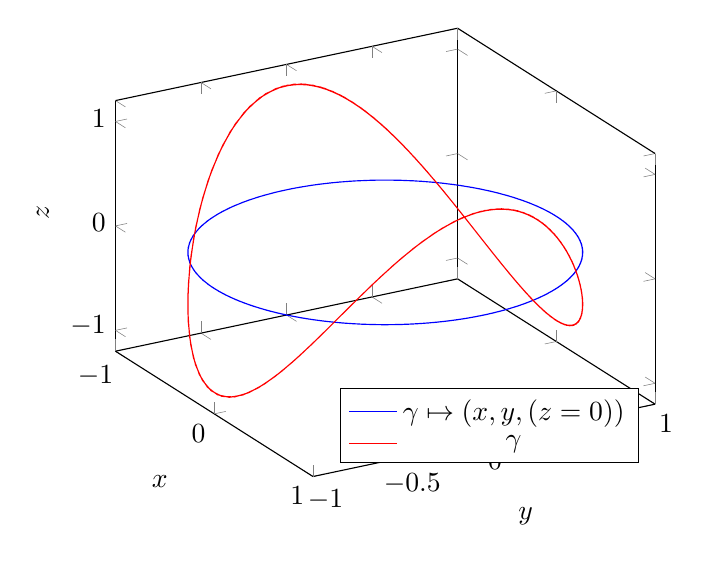
\begin{tikzpicture}
      \begin{axis}[
        view={60}{30},
        legend pos=south east,
        xlabel={$x$},
      	ylabel={$y$},
      	zlabel={$z$},]
        \addplot3[domain=0:5*pi,samples=150,samples y=0,color=blue]
          ({sin(deg(x))},
           {cos(deg(x))},
           {0});
        \addlegendentry{$\gamma \mapsto (x,y,(z=0))$}
        \addplot3[domain=0:5*pi,samples=150,samples y=0,color=red]
         ({cos(deg(x))},
          {sin(deg(x))},
          {cos(deg(x))^2 - sin(deg(x))^2});
        \addlegendentry{$\gamma$}
      \end{axis}
    \end{tikzpicture}
  \end{center}

  Wissen schonmal, dass $\gamma$ geschlossen ist, weil $\gamma(0) = \gamma(2\pi)$.

  Weiter betrachten wir:
  $$\begin{aligned}
    F: \R^3 & \to \R^3 \\
    \begin{pmatrix}
      x \\ y \\z
    \end{pmatrix} & \mapsto \begin{pmatrix}
      yz + \cos(x) \\ xz + \sin(y) \\ 2xy
    \end{pmatrix}
  \end{aligned}$$
  Wir berechnen
  $$\begin{aligned}
    \int_\gamma F dt & = \int_0^{2\pi} <F(\gamma_(\vartheta)),\gamma'(\vartheta)> d \vartheta \\
    & = \int_0^{2\pi} \left< \begin{pmatrix}
      \sin(\vartheta) (\cos(\vartheta)^2 - \sin(\vartheta)^2) + \cos(\cos(\vartheta)) \\
      \vdots \\ \vdots
    \end{pmatrix} , \begin{pmatrix}
      -\sin(\vartheta) \\ \cos(\vartheta) \\ \vdots
    \end{pmatrix} \right> d \vartheta
  \end{aligned}$$
  was wir leider nicht mehr berechnen können.

  Betrachten wir diese Kurve doch lieber als den Rand einer Fläche. Dann sagt der Satz von Stokes:

  Das Arbeitsintegral von $F$ entlang $\gamma$ lässt sich auch ausdrücken als das Integral von $rot(F)$ auf einer Fläche, deren Rand $\gamma$ ist.

  Es bietet sich an die Mannigfaltigkeit $M := \{(x,y,z) \in \R^3 \mid z = x^2 -y^2\}$ zu betrachten, und daraus die Fläche
  $$S := \{(x,y,z) \in \R^3 \mid z = x^2 -y^2 \land x^2 + y^2 \leq \}$$
  zu nehmen. ($M$ ist also die Fortsetzung von $S$).
  $$\begin{aligned}
    \int_\gamma F dt & \stackrel{\scriptscriptstyle Stokes}{=} \int_S rot(F) dn \\
    & \psi : \R^2 \to M \subseteq \R^3 \quad \psi(x,y) = (x,y,x^2 - y^2) \\
    & rot(F(x,y,z)) = \begin{pmatrix}
      \partial_2 F_3 - \partial_3 F_2 \\ -\partial_1 F_3 + \partial_3 F_1 \\ \partial_1 F_2 - \partial_2 F_1
    \end{pmatrix} = \begin{pmatrix}
      2x - x \\ -2y + y \\ z - z
    \end{pmatrix} = \begin{pmatrix}
      x \\ -y \\ 0
    \end{pmatrix} \\
    & = \int_B <rot(F)(\psi(x,y)),\partial_1 \psi \times \partial_2 \psi> d(x,y) \\
    & \text{mit } B := \{(x,y) \in \R^2 \mid x^2 + y^2 \leq 1\} \\
    & =\int_B \left<\begin{pmatrix}
      x \\ -y \\ 0
    \end{pmatrix}, \begin{pmatrix}
      1 \\ 0 \\2x
    \end{pmatrix} \times \begin{pmatrix}
      0 \\ 1 \\ -2y
    \end{pmatrix}\right> d(x,y) \\
    & \stackrel{\scriptscriptstyle elegant}{=} \int_B \det\begin{pmatrix}
      x & 1 & 0 \\ -y & 0 & 1 \\ 0 & 2x & -2y
    \end{pmatrix} d(x,y) \\
    & = \dots \\
    & \text{lang, \textbf{aber} berechenbar}
  \end{aligned}$$
\end{Beispiel}

\end{document}
